\documentclass[hyperref, a4paper]{article}

\usepackage{geometry}
\usepackage{titling}
\usepackage{titlesec}
% No longer needed, since we will use enumitem package
% \usepackage{paralist}
\usepackage{enumitem}
\usepackage{footnote}
\usepackage{enumerate}
\usepackage{amsmath, amssymb, amsthm}
\usepackage{mathtools}
\usepackage{bbm}
\usepackage{cite}
\usepackage{graphicx}
\usepackage{subfigure}
\usepackage{physics}
\usepackage{tensor}
\usepackage{siunitx}
\usepackage[version=4]{mhchem}
\usepackage{tikz}
\usepackage{xcolor}
\usepackage{listings}
\usepackage{autobreak}
\usepackage[ruled, vlined, linesnumbered]{algorithm2e}
\usepackage{nameref,zref-xr}
\zxrsetup{toltxlabel}
\usepackage[colorlinks,unicode]{hyperref} % , linkcolor=black, anchorcolor=black, citecolor=black, urlcolor=black, filecolor=black
\usepackage[most]{tcolorbox}
\usepackage{prettyref}

% Page style
\geometry{left=3.18cm,right=3.18cm,top=2.54cm,bottom=2.54cm}
\titlespacing{\paragraph}{0pt}{1pt}{10pt}[20pt]
\setlength{\droptitle}{-5em}
%\preauthor{\vspace{-10pt}\begin{center}}
%\postauthor{\par\end{center}}

% More compact lists 
\setlist[itemize]{
    itemindent=17pt, 
    leftmargin=1pt,
    listparindent=\parindent,
    parsep=0pt,
}

% Math operators
\DeclareMathOperator{\timeorder}{\mathcal{T}}
\DeclareMathOperator{\diag}{diag}
\DeclareMathOperator{\legpoly}{P}
\DeclareMathOperator{\primevalue}{P}
\DeclareMathOperator{\sgn}{sgn}
\newcommand*{\ii}{\mathrm{i}}
\newcommand*{\ee}{\mathrm{e}}
\newcommand*{\const}{\mathrm{const}}
\newcommand*{\suchthat}{\quad \text{s.t.} \quad}
\newcommand*{\argmin}{\arg\min}
\newcommand*{\argmax}{\arg\max}
\newcommand*{\normalorder}[1]{: #1 :}
\newcommand*{\pair}[1]{\langle #1 \rangle}
\newcommand*{\fd}[1]{\mathcal{D} #1}
\DeclareMathOperator{\bigO}{\mathcal{O}}

% TikZ setting
\usetikzlibrary{arrows,shapes,positioning}
\usetikzlibrary{arrows.meta}
\usetikzlibrary{decorations.markings}
\tikzstyle arrowstyle=[scale=1]
\tikzstyle directed=[postaction={decorate,decoration={markings,
    mark=at position .5 with {\arrow[arrowstyle]{stealth}}}}]
\tikzstyle ray=[directed, thick]
\tikzstyle dot=[anchor=base,fill,circle,inner sep=1pt]

% Algorithm setting
% Julia-style code
\SetKwIF{If}{ElseIf}{Else}{if}{}{elseif}{else}{end}
\SetKwFor{For}{for}{}{end}
\SetKwFor{While}{while}{}{end}
\SetKwProg{Function}{function}{}{end}
\SetArgSty{textnormal}

\newcommand*{\concept}[1]{{\textbf{#1}}}

% Embedded codes
\lstset{basicstyle=\ttfamily,
  showstringspaces=false,
  commentstyle=\color{gray},
  keywordstyle=\color{blue}
}

% Reference formatting
\newrefformat{fig}{Figure~\ref{#1}}

% Color boxes
\tcbuselibrary{skins, breakable, theorems}
\newtcbtheorem[number within=section]{warning}{Warning}%
  {colback=orange!5,colframe=orange!65,fonttitle=\bfseries, breakable}{warn}
\newtcbtheorem[number within=section]{note}{Note}%
  {colback=green!5,colframe=green!65,fonttitle=\bfseries, breakable}{note}
\newtcbtheorem[number within=section]{info}{Info}%
  {colback=blue!5,colframe=blue!65,fonttitle=\bfseries, breakable}{info}

\newenvironment{shelldisplay}{\begin{lstlisting}}{\end{lstlisting}}

\newcommand{\address}[1]{\href{#1}{\url{#1}}}

\title{Homework 8}
\author{Jinyuan Wu}

\begin{document}

\maketitle

\paragraph{Problem 1} Consider a 1D chain of identical atoms with one atom per unit cell. Each atom donates $Z$ electrons to the band structure. How many bands will be filled by electrons and briefly explain why?

\paragraph{Solution} When the bands overlap with each other,
we really can't say much about how many bands are filled,
because we can distort the bands and make the number of filled bands 
as many as we want (\prettyref{fig:overlap}).

\begin{figure}
    \centering
    \begin{tikzpicture}[x=0.75pt,y=0.75pt,yscale=-0.8,xscale=0.8]
    %uncomment if require: \path (0,300); %set diagram left start at 0, and has height of 300
    
    %Straight Lines [id:da4138677847824037] 
    \draw    (122,238) -- (311.5,238) ;
    \draw [shift={(313.5,238)}, rotate = 180] [fill={rgb, 255:red, 0; green, 0; blue, 0 }  ][line width=0.08]  [draw opacity=0] (12,-3) -- (0,0) -- (12,3) -- cycle    ;
    %Straight Lines [id:da19072401139926076] 
    \draw    (217.75,238) -- (217.75,55.85) ;
    \draw [shift={(217.75,53.85)}, rotate = 90] [fill={rgb, 255:red, 0; green, 0; blue, 0 }  ][line width=0.08]  [draw opacity=0] (12,-3) -- (0,0) -- (12,3) -- cycle    ;
    %Curve Lines [id:da6883784396806765] 
    \draw    (139.5,171) .. controls (173.5,170.85) and (190,225.15) .. (217.75,226) .. controls (245.5,226.85) and (255.5,170.85) .. (295.5,171) ;
    %Straight Lines [id:da37445061519997136] 
    \draw  [dash pattern={on 0.84pt off 2.51pt}]  (140,238) -- (140,53.85) ;
    %Straight Lines [id:da5423933952599624] 
    \draw  [dash pattern={on 0.84pt off 2.51pt}]  (295.5,238) -- (295.5,53.85) ;
    %Curve Lines [id:da04733929208931942] 
    \draw    (139.5,136) .. controls (173.5,135.85) and (190,214.15) .. (217.75,215) .. controls (245.5,215.85) and (255.5,135.85) .. (295.5,136) ;
    %Curve Lines [id:da41552926054468076] 
    \draw    (139.5,111) .. controls (173.5,110.85) and (190,203.15) .. (217.75,204) .. controls (245.5,204.85) and (255.5,110.85) .. (295.5,111) ;
    %Straight Lines [id:da9886126440781515] 
    \draw [color={rgb, 255:red, 74; green, 144; blue, 226 }  ,draw opacity=1 ]   (139.5,195) -- (295.5,195) ;
    
    % Text Node
    \draw (297.5,195) node [anchor=west] [inner sep=0.75pt]    {$\epsilon _{\text{F}}$};
    % Text Node
    \draw (315.5,238) node [anchor=west] [inner sep=0.75pt]    {$k$};
    
    
    \end{tikzpicture}
    
    \caption{Overlapping bands and partial filling}
    \label{fig:overlap}
\end{figure}

When there is no overlapping,
if $Z$ is even, then there are $Z/2$ bands filled,
because a band can host $N$ orbital modes 
and therefore it can host $2N$ electrons when spin is considered.
There are $ZN$ electrons in the band structure in total,
so we need $ZN / 2N = Z/2$ bands.
If $Z$ is odd, then we need to fill $(Z+1)/2$ bands,
because $N(Z-1)$ electrons are hosted by $(Z-1)/2$ bands,
and we need an additional band to host the rest $N$ electrons.

\paragraph{Problem 2} Consider a 1D system of a finite number of identical atoms $N$ arranged in a large ring $(N \gg 1)$. The circumference of the ring is $L=N a$ where $a$ is the primitive lattice constant. Below is a plot of the band structure in the Brillouin zone for this system when we employ the "empty lattice" (i.e., free electron; i.e., no periodic potential from the nuclei) approximation.
(a) What is the value of the minimum allowed wavevector $k_1\left(k_1>0\right)$ ?
What is the zone-edge wavevector $k_2$ ? What are the energies $E^{\prime}$ and $E^{\prime \prime}$ ?
(b) What are the velocity and effective mass associated with point $\alpha$ which lies at wavevector $k_2 / 2$ ?
(c) How many electrons can band 1 accommodate? Band 2?
(d) Redraw the figure when a weak potential is introduced from the ions.
(e) Will the answer to (b) change in the case of a weak potential? Why?

\begin{center}
    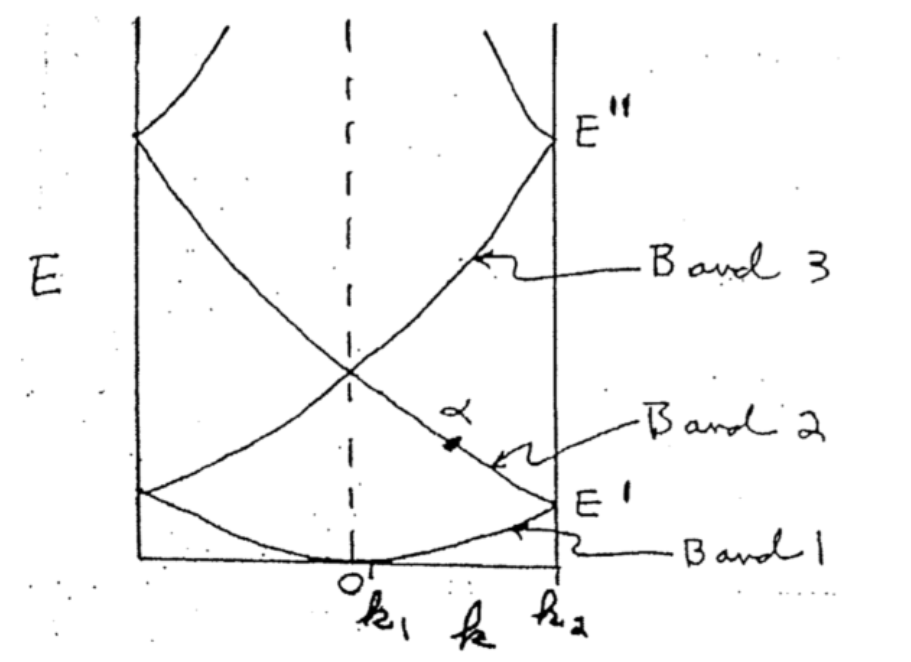
\includegraphics[width=0.6\textwidth]{bands/free-electron-folding-1.PNG}
\end{center}

\paragraph{Solution} \begin{itemize}
\item[(a)] We have 
\begin{equation}
    k_1 = \frac{2\pi}{L} = \frac{2\pi}{Na}, \quad 
    k_2 = \frac{\pi}{a}.
\end{equation}
\begin{equation}
    E' = \frac{\hbar^2}{2m} \left(\frac{\pi}{a}\right)^2.
\end{equation}
\begin{equation}
    E'' = \epsilon_{n = 3, \vb*{k} = \pi / a} = \frac{\hbar^2}{2m} \Big( 
        \frac{\pi}{a} + \underbrace{\frac{2\pi}{a}}_{\vb*{G}_{n = 3}} \Big)
        = 9 \frac{\hbar^2}{2m} \left(\frac{\pi}{a}\right)^2.
\end{equation}

\item[(b)] From the band diagram, 
\begin{equation}
    \epsilon_{n = 2, k} = \frac{\hbar^2}{2m} (k + G_2)^2 
    = \frac{\hbar^2}{2m} \left( k - \frac{2\pi}{a} \right)^2.
\end{equation}
The group speed is 
\begin{equation}
    v = \frac{1}{\hbar} \pdv{\epsilon_{n = 2, k}}{k} = \frac{\hbar}{m} \left( k - \frac{2\pi}{a} \right)
    = - \frac{3 \hbar \pi}{2 m a}.
\end{equation}
The effective mass is 
\begin{equation}
    \frac{1}{m^*} = \frac{1}{\hbar^2} \pdv[2]{\epsilon_{n = 2, k}}{k}
    = \frac{1}{m}, \quad m^* = m.
\end{equation}

\item[(c)] Regardless of the shape,
each band accommodates 
\begin{equation}
    \underbrace{2}_{\text{spin}} \cdot \frac{2 k_2}{k_1} = 2N
\end{equation}
electrons.

\item[(d)] See \prettyref{fig:weak-perturbation}.

\begin{figure}
    \centering
    \begin{tikzpicture}[x=0.75pt,y=0.75pt,yscale=-1,xscale=1]
    %uncomment if require: \path (0,416); %set diagram left start at 0, and has height of 416
    
    %Straight Lines [id:da7072007796490802] 
    \draw    (223,377) -- (406,377) -- (474,377) ;
    \draw [shift={(476,377)}, rotate = 180] [fill={rgb, 255:red, 0; green, 0; blue, 0 }  ][line width=0.08]  [draw opacity=0] (12,-3) -- (0,0) -- (12,3) -- cycle    ;
    %Straight Lines [id:da27738069282968025] 
    \draw    (352,390.67) -- (352,113) ;
    \draw [shift={(352,111)}, rotate = 90] [fill={rgb, 255:red, 0; green, 0; blue, 0 }  ][line width=0.08]  [draw opacity=0] (12,-3) -- (0,0) -- (12,3) -- cycle    ;
    %Straight Lines [id:da7881533185962195] 
    \draw  [dash pattern={on 4.5pt off 4.5pt}]  (293,124) -- (293,377) ;
    %Straight Lines [id:da7005644131540305] 
    \draw  [dash pattern={on 4.5pt off 4.5pt}]  (412,124) -- (412,377) ;
    %Curve Lines [id:da014879760018285948] 
    \draw    (293,358.67) .. controls (309.46,358.08) and (315.46,376.5) .. (352,377) ;
    %Curve Lines [id:da5056941741539491] 
    \draw    (411,358.67) .. controls (396.21,358.58) and (387.96,377.08) .. (352,377) ;
    %Curve Lines [id:da6865802022984844] 
    \draw    (293,351.67) .. controls (327,350.67) and (338.71,304.92) .. (352,305.67) ;
    %Curve Lines [id:da7066378119938326] 
    \draw    (411,351.67) .. controls (377,350.67) and (364,305.67) .. (352,305.67) ;
    %Curve Lines [id:da8127590172034278] 
    \draw    (293,213.67) .. controls (310.96,213.42) and (336.96,298.92) .. (352,298.67) ;
    %Curve Lines [id:da6250242912054444] 
    \draw    (411,213.67) .. controls (397.46,212.17) and (364.71,298.67) .. (352,298.67) ;
    %Curve Lines [id:da7990024333659946] 
    \draw    (293,205.67) .. controls (302.96,206) and (313.21,167) .. (318,124.67) ;
    %Curve Lines [id:da4293644587297756] 
    \draw    (412,205.67) .. controls (402.21,206) and (390.46,169.08) .. (384,124.67) ;
    
    % Text Node
    \draw (478,377) node [anchor=west] [inner sep=0.75pt]    {$k$};
    % Text Node
    \draw (352,108) node [anchor=south] [inner sep=0.75pt]    {$\epsilon _{k}$};
    
    
    \end{tikzpicture}
    
    \caption{Empty lattice model after weak perturbation}
    \label{fig:weak-perturbation}
\end{figure}

\item[(e)] Of course there will be small changes, but not very significant:
In first-order correction to band energy,
we have 
\begin{equation}
    \Delta \epsilon_{\vb*{k}} = \mel{\vb*{k}}{V}{\vb*{k}}
    = \frac{N}{V} \int_{\text{u.c.}} \dd[2]{\vb*{r}} U(\vb*{r}),
\end{equation}
which doesn't have any $\vb*{k}$ dependency.
So a weak potential field just gives all bands a small, constant shift,
and the derivatives of $\epsilon_{\vb*{k}}$ all stay the same,
and so is the case for group velocity or $m^*$.

\end{itemize}

\paragraph{Problem 3} Consider the two-dimensional square lattice with lattice constant $a$ where the crystal potential is
$$
U(x, y)=-4 A \cos \left(\frac{2 \pi x}{a}\right) \cos \left(\frac{2 \pi y}{a}\right) .
$$
Assuming $\mathrm{U}$ is a weak potential, compute the energy gap at the corner point of the Brillouin zone $\left(\frac{\pi}{a}, \frac{\pi}{a}\right)$ to the lowest order in $A$. (You should only be diagonalizing a $2 \times 2$ matrix. First, find all the degenerate free electron states at that point in the BZ. Second, see which ones connect via the potential and build the $2 \times 2$ problem.)

\paragraph{Solution} We first evaluate the hopping matrix.
We have ($V = N a^2$ is the total area of the crystal; 
it should be $A$ but it's in conflict with the strength of the potential)
\begin{equation}
    \begin{aligned}
        \mel{\vb*{k}'}{U}{\vb*{k}} 
        &= \int \dd[2]{\vb*{r}} \frac{1}{\sqrt{V}} \ee^{- \ii \vb*{k}' \cdot \vb*{r}} U(\vb*{r}) 
        \frac{1}{\sqrt{V}} \ee^{\ii \vb*{k} \cdot \vb*{r}} \\
        &= \frac{N}{V} \sum_{\vb*{G}} \delta_{\vb*{k}', \vb*{k} + \vb*{G}}
        \int_{\text{u.c.}} \dd[2]{\vb*{r}} \ee^{- \ii \vb*{G} \cdot \vb*{r}} U(\vb*{r}) \\
        &= \frac{N}{V} \sum_{\vb*{G}} \delta_{\vb*{k}', \vb*{k} + \vb*{G}}
        \int_0^a \dd{x} \int_0^a \dd{y} \ee^{- \ii \frac{2\pi}{a} n_x x} \ee^{- \ii \frac{2\pi}{a} n_y y}
        (-4 A) \cos(\frac{2\pi x}{a}) \cos(\frac{2\pi y}{a}) \\
        &= - 4 A \frac{N}{V} \sum_{\vb*{G}} \delta_{\vb*{k}', \vb*{k} + \vb*{G}} 
        \cdot \frac{a}{2} (\delta_{n_x, 1} + \delta_{n_x, -1}) 
        \cdot \frac{a}{2} (\delta_{n_y, 1} + \delta_{n_y, -1}) \\
        &= - A \sum_{\vb*{G}} \delta_{\vb*{k}', \vb*{k} + \vb*{G}} \sum_i \delta_{\vb*{G} \vb*{G}_i},
    \end{aligned}
\end{equation}
where 
\begin{equation}
    \vb*{G}_i = \frac{2\pi}{a} (\pm 1, \pm 1). 
\end{equation}
The four $\vb*{G}_i$ points can be transformed into each other by symmetric operations,
and without loss of generality,
below we just consider $\vb*{G}_1 = \frac{2\pi}{a} (1, 1)$.

The four corners of the Brillouin zone constitute a degeneracy subspace.
With $\vb*{G}_1$, 
$\frac{\pi}{a} (1, 1)$ and $\frac{\pi}{a} (-1, -1)$ are connected.
So the Hamiltonian for the two-state subspace is 
\begin{equation}
    \pmqty{
        \frac{\hbar^2}{2m} \cdot 2 \frac{\pi^2}{a^2} & - A \\
        - A & \frac{\hbar^2}{2m} \cdot 2 \frac{\pi^2}{a^2} 
    },
\end{equation}
and the eigenvalues -- the energies after correction -- are 
\begin{equation}
    E = \frac{\hbar^2}{m} \frac{\pi^2}{a^2} \pm A,
\end{equation}
so the energy gap is $2A$.

\paragraph{Problem 4} A pure crystalline material with no impurity or dopants appears transparent but colored in the following sense: if you hold it up to white light, the light transmitted through it looks red but you can see clearly through it otherwise (as if it was red colored glass).
(a) Is this material a conductor or insulator (at $\mathrm{T}=0)$ ?
(b) What is the approximate (direct) band gap of this material in eV?

\paragraph{Solution} \begin{itemize}
\item[(a)] It has to be an insulator.
Selective absorption of light of one particular color 
means there is a direct band gap corresponding to the energy 
of the photon of that color.
\item[(b)] The transmitted light is red, 
so light that is not red is absorbed,
so the direct band gap -- the minimum energy of absorbed photon -- 
is around \SI{2}{eV}.
\end{itemize}

\paragraph{Problem 5} Below you find schematics of the key aspects of three unidentified pure crystalline materials that have fundamental energy gaps and are thus insulating at $\mathrm{T}=0$. In all three diagrams, $\mathrm{k}$ (wave vector) is horizontal and energy is vertical; the horizontal line is the top of the valence band (highest occupied energy level); and all the low-energy band edge differences are shown with numerical values.
a) Which material is best for use as an LED that generates visible light? Roughly what color LED will it be?
b) Which material becomes a thermally activated conductor at the lowest temperature (i.e., its conductivity "turns on" first as we increase temperature from $\mathrm{T}=0)$ ? Increasing temperature will energize electrons to leave what used to be filled states at $\mathrm{T}=0$ and go into what used to be empty states; then the bands become partially occupied and we can have conduction.

\paragraph{Solution} \begin{itemize}
\item[(a)] We just need to find a material whose direct band gap falls in the visible light spectrum.
This is the third material ($E_g = \SI{1.42}{eV}$), 
and it will be a red color LED.
\item[(b)] The smaller the direct band gap is, 
the easier it is to be a thermally activated conductor.
So the conductivity of the second material ($E_{g} = \SI{0.35}{eV}$) 
turns on first.
\end{itemize}

\end{document}